\documentclass{article}
\usepackage{graphicx}
\usepackage{amsmath}

% This package allows us to write text in color
\usepackage{xcolor}

% if you need to pass options to natbib, use, e.g.:
%     \PassOptionsToPackage{numbers, compress}{natbib}
% before loading neurips_2018

% ready for submission
% \usepackage{neurips_2018}

% to compile a preprint version, e.g., for submission to arXiv, add add the
% [preprint] option:
%     \usepackage[preprint]{neurips_2018}

% to compile a camera-ready version, add the [final] option, e.g.:
     \usepackage[final]{neurips_2018}

% to avoid loading the natbib package, add option nonatbib:
%     \usepackage[nonatbib]{neurips_2018}

\usepackage[utf8]{inputenc} % allow utf-8 input
\usepackage[T1]{fontenc}    % use 8-bit T1 fonts
\usepackage{hyperref}       % hyperlinks
\usepackage{url}            % simple URL typesetting
\usepackage{booktabs}       % professional-quality tables
\usepackage{amsfonts}       % blackboard math symbols
\usepackage{nicefrac}       % compact symbols for 1/2, etc.
\usepackage{microtype}      % microtypography

\title{Drought Analysis}

\author{%
  Xingyao Chen\\
  Harvey Mudd College\\
  \texttt{xchen@hmc.edu} \\
  \And
  Cassidy L\^e\\
  Harvey Mudd College\\
  \texttt{cle@hmc.edu} \\
}

\begin{document}

\maketitle

\begin{abstract}
  Drought has long affected the United States well past the 21\textsuperscript{st} century, and it does so in many aspects. It not only impacts the everyday lives of average Americans, but it also greatly cripples numerous industries, such as agriculture, technology, consumer discretionary, and consumer staples. In this paper, we used machine learning techniques to analyze the effect of drought on industry earnings per county. [1-2 sentences about results]
\end{abstract}

\section{Background and Significance}
% Background info on drought in the U.S.
According to Merriam-Wesbter, drought is defined as a period of dryness especially when prolonged. Droughts are relative, meaning that "normal" conditions vary from region to region which, in affect, changes the qualifications for drought from region to region. Additionally, there are many levels of drought severity. For consistency, we will use the intensity levels defined by the Drought Monitor: None is no drought, D0 is abnormally dry, D1 is moderate drought, D2 is severe drought, D3 is extreme, and D4 is exceptional drought.

For about a decade now, the U.S. has experienced numerous droughts at different levels of severity. Between June 2011 and October 2011, the U.S. experienced exceptional drought (D4) over the largest land area of greater than 9\%. In August 2012, extreme (D3) and exceptional drought (D4) extended over 20\% of the U.S. The following month, 55\% of the U.S. experienced drought of at least moderate intensity (D1) while 35\% was under severe drought (D2) conditions. In contrast, in May 2017, "only 3.8\% of the total U.S. land area was affected by drought of at least moderate intensity (D1)." \cite{Folger:2017jd}

% Background info on industries in the U.S.
Droughts affect numerous industries in the U.S., most notably agriculture. In California, 80\% of fresh water withdrawals goes to agricultural uses while the remaining 20\% are for urban uses for households and nonfarm businesses.\cite{Kearney:2014} However, there are many other industries that are impacted other than agriculture. For example, the technology industry relies heavily on water as a cooling mechanism because of its high capacity to absorb heat. Additionally, water is often used for power generation. In fact, approximately 49\% of total water withdrawals in the U.S. went to power generation in 2005. Some other industries that heavily rely on water, though less obviously, are the consumer discretionary sector, which includes Starbucks and Best Buy, as well as the consumer staples sector, which consists of Walmart and Whole Foods.\cite{Kearney:2014} Taken from the 2010 U.S. Geological Survey, the national estimated use of water by industry in each U.S. state and territory is graphically represented by \textbf{Figure \ref{fig:label1}}.\cite{USGS:2010}
\begin{figure}[hbt!]
    \centering
    \includegraphics[width=15cm]{WaterUsageFigure}
    \caption{Water usage by state and industry 2010.}
    \label{fig:label1}
\end{figure}


The scarcity of available water resources to provide for the needs of various regions around the world is set to reach an unprecedented and distressing level in the coming decades.  This may sound like a topic better reserved for environmental analysts, but to be clear, there are considerable stakes at play.  The severity of the situation is set to affect more than just the world economy;water  scarcity  and  its  symptoms  may  very  well  contribute  to  increasing  sociopolitical  and  international conflicts, as suffering nations begin to question the distribution of fresh water resources.  Furthermore, the increasing effects of climate change are cause for concern regarding the stability and dependability of water resources in the coming decades.  Though there exist a deluge of data relevant to the use of and economics surrounding water, the unpredictability of water availability creates a nontrivial statistical task in building an understanding the crisis.  In order to reason intelligently about the potential calamities of water availability,it  is  necessary  to  develop  a  precise  notion  of  ‘sensitivity’ with  respect  to  entities  on  the  level  of  nation, state, or county.  Ultimately we invest in the use of statistical methods and machine learning to inform the actions we take in combating the near and far term effects of crises.  That said, policies are enacted  in  a  setting  in  which  the  resources  necessary  to  take  action  are  limited.   Providing  a  compelling survey  of  where  we  ought  to  divert  attention  and  resources  is  a  necessary  component  of  any  successful strategy.  \\

To that end, we investigated the economical changes caused by a significant fluctuation in drought level 
in a particular county. To answer the question we proposed, we modularized our investigation into 3 steps. First, we clustered U.S. counties based on their 
sources of income such that counties with similar economies are groups together. All future analyses are conducted within each county cluster to in order to account for differences between clusters. Second, we measured the effect of drought levels on several water withdraw categories. We conclude by modeling how much 
a county's total median earnings is influenced by changes in water withdraw. 


\section{Data set}
% Just an overview of where we got the data and what it contains
The data we used is taken from the following three different data sets: \texttt{droughts}, \texttt{earnings}, and \texttt{water\_usage}.

\texttt{droughts} is sourced by the U.S. Drought Monitor. It contains the particular percentage of various range of drought severities, indexed by counties for particular start-end periods throughout the United States. This data set consists of 1.35 million rows and 11 columns.

\texttt{earnings} is sourced by the U.S. Census. It contains the industry-specific mean earnings (in that year's U.S. dollars and adjusted for inflation) indexed by county between 2010-2016. This data set consists of 21,999 rows and 31 columns.

\texttt{water\_usage} is sourced by the U.S. Department of the Interior. It contains information about particular water usage (irrigation, public supply, crop, etc.) and thermoelectric power generated for counties that were found in the year 2010.  This data set consists of 3,225 rows and 23 columns.

\section{Methods}
We used the following three methods to analyze and model our data set: $k$-Means Clustering, Linear Regression Modeling, and Ridge Regression Modeling with Cross Validation (CV).

% KMeans Clustering
\subsection{Clustering based on industry}
\subsubsection{Purpose of clustering based on industry}
The \texttt{earnings} data set provides information on the total earnings for a certain industry in a given county in the Untied States. Specifically, each data point in this set is a numerical value that is associated with a specific industry as well as a distinct county in the U.S. Using $k$-Means Clustering, which is further explained in the next sub-sub-section \textbf{3.1.2}, we grouped these data points into clusters based on the value of \texttt{earnings} in U.S. dollars (USD). This creates clusters that essentially represent different industries in the U.S. Furthermore, each cluster consists of various points that each represent a distinct county in the U.S. With the resulting clusters, we were then able to analyze drought's effect on water usage, which is outlined in sub-section \textbf{3.2}, as well as model the median earning with water usage, which is outlined in sub-section \textbf{3.3}.
\subsubsection{Background and implementation of $k$-Means Clustering}
% Background of KMeans Clustering
The $k$-Means algorithm clusters data by separating samples into groups of equal variance, minimizing the within-cluster sum of squares (WCSS) of each cluster. Specifically, the $k$-Means algorithm partitions a set of $n$ samples into $k$ disjoint clusters, in which each sample belongs to the cluster with the nearest mean $\mu_j$. Therefore, each cluster $j=1,...,k$ has a corresponding mean $\mu_j$, which is called a "centroid". Ideally, the algorithm chooses centroids that minimize the WCSS for its corresponding cluster.\cite{sklearnKMeans:2018} Given a set of $n$ samples $X=\{x_1,x_2,...,x_n\}$ that are partitioned into the set of $k$ clusters $C=c_1,c_2,...,c_k$. Then, the WCSS is defined as
\begin{equation}
    \sum_{i=0}^n\min_{\mu_j\in C}\bigg(||x_i-\mu_j||^2\bigg).
\end{equation}
% Implementation of KMeans Clustering
In order to implement the $k$-Means algorithm, we used the built-in Python tool \texttt{sklearn}, which has a $k$-Means algorithm called \texttt{sklearn.cluster.KMeans}. This algorithm has parameters \texttt{n\_clusters}, which indicates how many clusters the sample will be partitioned into, \texttt{n\_init}, which represents the number of times the algorithm will be run with different centroid seeds to determine the best output (based on the best WCSS), and \texttt{random\_state}, which represents the number of random generations for centroid initialization.\cite{KMeans:2018}

%Implementation of KMeans Clustering
For our data set, we used 5 clusters because there were 12 listed distinct industries where some overlapped. The industries are the following: agriculture, forestry, fishing and hunting, and mining; construction; manufacturing; wholesale trade; retail trade; transportation and warehousing, and utilities; information; finance and insurance, and real estate and rental and leasing; professional, scientific, and management, and administrative and waste management; educational services, and health care and social assistance; arts, entertainment, and recreation, and accommodations and food services; public administration. Consequently,  we only used approximately half the number of distinct industries. These industries were used as the features for the algorithm.

% Linear Regression
\subsection{Analysis of drought's effect on water usage}
\subsubsection{Purpose of drought's effect on water usage analysis}
In our analysis of drought's effect on water usage, we analyzed the clusters that were produced from implementing the $k$-Means algorithm. For each cluster, we analyzed the relationship between its associated \textt{drought} data and its associated \textt{water\_usage} data using linear regression. The results of this analysis produce a linear regression equation that reflects how heavily each cluster's drought affects the overall water usage.

Knowing the relationship between \textt{drought} and \textt{water\_usage}, we can then determine the correlation between \textt{drought} and the economy. This can be done by first analyzing the relationship between \textt{water\_usage} and \textt{earnings}, which is done in the next sub-section \textbf{3.3}.

\subsubsection{Background and implementation of Linear Regression}
% Background of Linear Regression
Linear regression fits a linear model to a data set. It does so by adjusting the set of parameters such that the model's sum of the squared residuals is minimized. The linear model is of the form
\begin{equation}
    y=\beta_1x_1+\beta_2x_2+...+\beta_nx_n,
\end{equation}
where $y$ is the target variable, $\{x_1,...,x_n\}$ represents the features, and $\{\beta_1,...,\beta_n\}$ represents the set of coefficients.\cite{sklearn:2019}

In the analysis of drought's effect on water usage, the target variable is the overall water usage and the features are the drought levels associated with each cluster. In other words, each $x_i$ corresponds to the associated drought level for a cluster $c_i$. Then, the coefficients represent the weights assigned to each feature.

%Implementation of Linear Regression 
In order to implement the Linear Regression Model, we used the built-in Python tool \texttt{sklearn}, which has a Linear Regression algorithm called \texttt{sklearn.linear\_model.LinearRegression}. First, we determined the average water usage for each cluster at a given drought level. We classified the drought level for each county  by selecting the highest drought level at which at least 10\% of the population was affected. Because there were five clusters, and each cluster has data for four different drought levels (D0, D1, D2, D3), there were a total of twenty means of water usage calculated. Then, for each cluster, the calculated average of water usage was fitted with its corresponding drought level to produce a linear regression model. This model represents the relationship between drought level and water usage.

% Ridge Regression CV
\subsection{Modeling of median earning with water usage}
\subsubsection{Purpose of modeling median earning with water usage}
In our modeling of the relationship between median earning and water usage, we analyzed the clusters that were produced from implementing the $k$-Means algorithm in sub-section \textbf{3.1}. For each cluster, we analyzed the relationship between its associated \texttt{water\_usage} data and its associated \textt{earnings} data using Ridge Regression with Cross Validation (CV). The results of this analysis produce a regression model with weights that reflect how heavily each cluster's water usage affects the overall median earnings. This can reveal how much of the economy in a given county will be hurt by a decrease in water usage. With this information as well as any findings from an analysis of drought's effect on water usage, we can determine the impact of drought on the economy.
\subsubsection{Background and implementation of Ridge Regression with CV}
% Background of Ridge Regression
Ridge Regression is used for analyzing multiple regression data when the data exhibits mulicollinearity. Multicollinearity occurs when independent variables have near-linear relationships. This results in large variances within the data, which may produce values that are far from the true value. For example, it can result in inaccurate estimates of the regression coefficients. Some other distortions include inflation of the standard errors of the regression coefficients, deflation of the partial t-tests for the regression coefficients, false or non-significant p-values, and degradation of the predictability of the. To mitigate the effects of multicollinearity, Ridge Regression adds a degree of bias to the regression estimates. This reduces the standard errors, which produces more reliable estimates.\cite{RidgeReg:2018}

Ridge Regression first requires the standardization of both independent and dependent variables. Then, ridge regression estimates the regression coefficients by minimizing the following:
\begin{equation} \label{RidgeRegEq}
    ||y-X\beta||_2^2+\lambda||\beta||_2^2
\end{equation}
where $||y-X\beta||_2^2$ is the sum of the squared residuals, $||\beta||_2^2$ is called the penalty, and $\lambda$ indicates the severity of the penalty. By minimizing the sum of the squared residuals plus the penalty, the Ridge Regression line adds a small amount of bias but also decreases the variance. Consequently, the results of Ridge Regression are not as sensitive to weight as those of other regression models, such as Least Squares Regression.\cite{RidgeReg:2018}

% Background on Cross Validation
In our implementation of Ridge Regression, we also included Cross Validation (CV). CV ensures that our results produced the best fit regression line. It does so by evaluating the accuracy of different combinations of training data and testing data, and uses the best method produced by the CV.

%Implementation of Ridge Regression
In order to implement Ridge Regression with CV, we used the built-in Python tool \texttt{sklearn}, which has a Ridge Regression with CV algorithm called \texttt{sklearn.linear\_model.RidgeCV}. This algorithm has parameters \texttt{alphas}, which is a set of $\lambda$ values to test with CV, \texttt{normalize}, which indicates whether to normalize the regressors prior to executing the regression analysis, and \texttt{cv}, which indicates how many iterations of Cross Validation to execute.

For our data set, the different $\lambda$ values we tested were $0.001, 0.1, 1, 10,$ and $100$. Additionally, we set the \texttt{normalize} parameter to \texttt{True} so that the algorithm would normalize the regressors. Finally, we decided to run eight different CVs.

\section{Results} 
\subsection{Industry Clustering}

\begin{figure}[hbt!]
    \centering
    \includegraphics[width = 0.6\textwidth]{manufacturingVutilities_kmeans.png}
    \caption{Visualization of counties grouped by K-Means Clustering, plotted over utility and manufacturing earning features.}
    \label{fig:cluster1}
\end{figure}
\begin{figure}[hbt!]
    \centering
    \includegraphics[width = 0.6\textwidth]{manufacturingVpub_admin_kmeans.png}
    \caption{Visualization of counties grouped by K-Means Clustering, plotted over public administration and manufacturing earning features.}
    \label{fig:cluster2}
\end{figure}
\begin{figure}[hbt!]
    \centering
    \includegraphics[width = 0.6\textwidth]{utilitiesVinformation_kmeans.png}
    \caption{Visualization of counties grouped by K-Means Clustering, plotted over utility and information earning features.}
    \label{fig:cluster3}
\end{figure}
K-Means clustering of U.S. counties yielded 5 clusters, 
with 145, 659, 502, 787, and 311 counties belonging to each respective cluster. Qualitatively, our clustering results indicate
that differences between county groups is most significantly explained by earnings in utilities, information, and manufacturing (\textbf{Fig. \ref{fig:cluster1}}, \textbf{Fig. \ref{fig:cluster2}}, \textbf{Fig. \ref{fig:cluster3}}).


\subsection{Effect of drought on water withdraw broken down categories}
From our analysis, we have determined that for a select number of withdraw categories, water withdraw  
decreased as the severity of drought increased. In particular, 
surface water withdraw decreased across the majority of clusters, followed by livestock, irrigation, aquaculture, and thermoelectric. 

Nonetheless, not every water withdraw category decreased with drought severity. This is expected because water reservoirs like groundwater is not affected by temporary drought. Also, it is unethical to restrict the withdraw of water to use for certain categories such as domestic supply. 

\begin{table}[htbp!]
  \caption{Significant coefficients of water withdraw vs. drought level regression model}
  \label{sample-table}
  \centering
  \begin{tabular}{l|l|lllll}
    \toprule
    
    &&&Clusters&&& \\
    % \hline
    \cmidrule(r){3-7}
           && 0     &1 & 2&3 & 4  \\
    \midrule
 Withdraw & thermoelectric    & $-1.01$ & - & - &  - & -\\
  Categories & surface-water   &$-0.326$  & - & $-0.340$ & $-0.332$ &$-0.343$\\
   & livestock &- & $-0.414$& - &$-0.472$& -\\
   & irrigation &-0.394&-&$-0.312$ &- & -\\
   & aquaculture &-&-&-&$-0.853$ & -\\
    \bottomrule
  \end{tabular}
\end{table}

\begin{figure}[htb!]
    \centering
    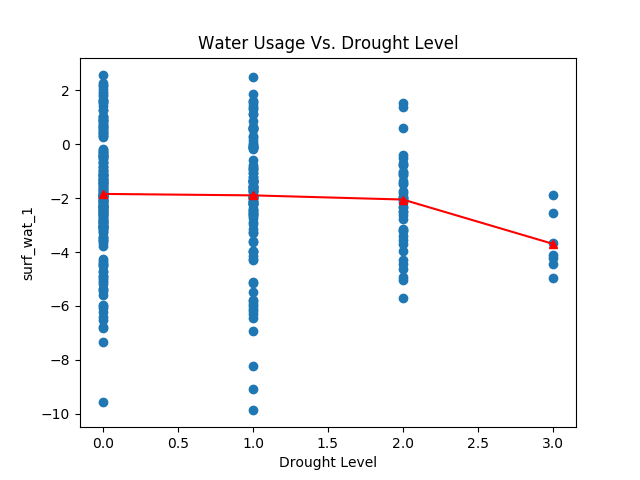
\includegraphics[width = 0.7\linewidth]{c2_surf_wat_1Veffect_d.png}
    \caption{Plot of surface-water withdraw (logged) vs. drought level for cluster 2 counties.}
    \label{fig:my_label}
\end{figure}

\begin{figure}[htb!]
    \centering
    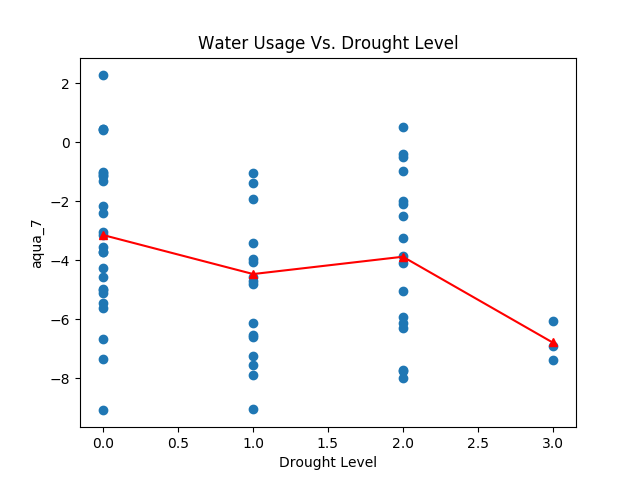
\includegraphics[width = 0.7\linewidth]{c4_aqua_7Veffect_d.png}
    \caption{Plot of aquaculture withdraws (logged) vs. drought level for cluster 3 counties.}
    \label{fig:my_label}
\end{figure}

\begin{figure}[t!]
    \centering
    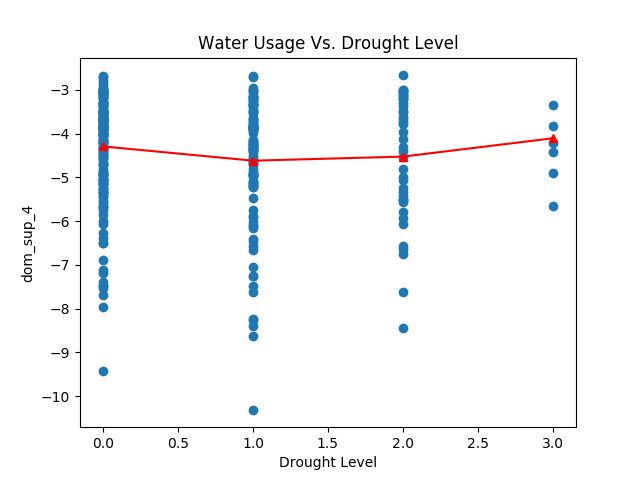
\includegraphics[width = 0.7\linewidth]{c2_dom_sup_4Veffect_d.png}
    \caption{Plot of surface-water withdraw (logged) vs. drought level for cluster 2 counties.}
    \label{fig:my_label}
\end{figure}

\clearpage

\subsection{Effect of water withdraw on county total median earning}


According to our regression model, increasing  
 the amount of water withdrawn for 
 specific categories yields an increase in total median earnings. Namely, water withdraw for industrial use and mining use had a large positive effect on median earnings for counties in clusters 1, 2, 3 and 4. In figures 8-12, 
 we present the top 2 water withdraw categories that has the most positive effect on median earnings for each of the 5 county clusters. 
 
 

\begin{table}[hbt!]
  \caption{Coefficients of median earnings vs. water withdraw ridge regression model}
  \label{sample-table}
  \centering
  \begin{tabular}{l|l|lllll}
    \toprule
    &&&Clusters&&& \\
    % \hline
    \cmidrule(r){3-7}
           && 0     &1 & 2&3 & 4  \\
    \midrule
 Withdraw & Public Supply   & -72.14   & 15.25  &   138.40  & -124.00 & 64.32 \\   
  Categories & Domestic   &  -15.08 & -9.23  & -0.06   &   34.21 & 3.93 \\
   & Industrial &  -30.45 & 53.27 & 121.12 &  255.10  &  201.32 \\
   & Irrigation & -619.02  & -78.26 &  -276.35 & 182.48 & -19.80 \\ 
   & Livestock &  -3.22& -55.30 &  -41.32  &   19.83 &  3.24\\
   & Aquaculture &  -139.70   &  -58.52 & 178.29  &    -1.79  &  -12.96\\  
   & Mining & -10.72  &  139.86   &  44.35 &  27.64 & 68.65 \\
   & Thermoelectric &  16.38  & 226.88 & -7.12 & -118.46  &  41.52  \\
   & groundwater & -716.07  &  24.90  &   113.76 &  -192.74 & -34.50  \\
   & surface-water &    -510.84 &  4.86 &  34.67 & -10.60 &  2.59\\
    \bottomrule
  \end{tabular}
\end{table}



\begin{figure}[hbt!]
    \centering
    \includegraphics[width = \linewidth]{linreg_c0.png}
    \caption{Plot of total median earning vs. water withdraw categories -- industrial and mining -- for cluster 0.}
    \label{fig:my_label}
\end{figure}



\begin{figure}[hbt!]
    \centering
    \includegraphics[width = \linewidth]{linreg_c1.png}
    \caption{Plot of total median earning vs. water withdraw categories -- thermoelectric and mining -- for cluster 1.}
    \label{fig:my_label}
\end{figure}



\begin{figure}[hbt!]
    \centering
    \includegraphics[width = \linewidth]{linreg_c2.png}
    \caption{Plot of total median earning vs. water withdraw categories -- aquaculture and public supply -- for cluster 2.}
    \label{fig:my_label}
\end{figure}



\begin{figure}[hbt!]
    \centering
    \includegraphics[width = \linewidth]{linreg_c3.png}
    \caption{Plot of total median earning vs. water withdraw categories -- industrial and irrigation -- for cluster 3.}
    \label{fig:my_label}
\end{figure}




\begin{figure}[hbt!]
    \centering
    \includegraphics[width = \linewidth]{linreg_c4.png}
    \caption{Plot of total median earning vs. water withdraw categories -- industrial and mining -- for cluster 4.}
    \label{fig:my_label}
\end{figure}

\clearpage
\section{Conclusion}
In Iran, "a 1\% decrease in precipitation below the long-run average results in a 0.68\% decline in the value added of the crops and horticulture sector." A 45\% decline from average precipitation caused an overall GDP drop by about 4.4\%. \cite{Salami:2008} In South Dakota, due to the drought in 2002, the agricultural income experienced a loss of \$829 million and a total economic loss of \$1,807 million. \cite{Diersen:2002}


% \subsubsection*{Acknowledgments}


\clearpage
% Could also try \newpage or \pagebreak
%--------------------
%	BIBLIOGRAPHY
%--------------------

\bibliographystyle{unsrt}

\bibliography{MidtermBib}

%----------------------------------------------------------------------------------------

\end{document}